
\chapter{基于容器的多终端透明计算迁移技术}\label{chap:computation_offloading}

\section{引言}

随着计算机技术的快速发展和边缘计算技术的逐渐成熟,位于网络边缘的用户终端设备在用户的数字化生活中正扮演着越来越重要的角色,其定位逐渐从单一的用户服务发起者向用户服务的提供者转变。这会使用户终端承担越来越多的计算任务,这也对终端设备的服务质量和计算能力提出了越来越高的要求。为了满足用户对于服务质量的要求,人们提出了计算迁移技术,将终端设备上的计算任务通过网络迁移到云端服务器上来完成。但是引入云端协同的计算迁移技术,还是存在着时延较大、数据隐私性不能保证、成本较高等问题,难以满足用户需求。而另一方面,边缘终端设备距离用户更近,而且拥有很多空余资源没有得到充分利用,如何将这部分距离用户更近、成本更低的资源组织利用起来为用户设备提供计算迁移服务也成为了计算迁移技术中的一个值得研究的问题。本文以HTML5中的Web Worker方法为例,研究Web应用透明计算迁移到以容器形式部署在边缘设备上的服务端,设计并实现了一种基于容器的Web Worker透明边缘计算迁移系统,并利用实验来验证该系统能够将周围设备的资源利用起来,减少计算总执行时间,提升用户体验。

本章的内容组织结构如下:第\ref{sec:computation_offloading_related_work}节介绍了计算迁移技术的相关研究工作,包括云计算中的计算迁移技术、基于Web Worker的计算迁移技术以及虚拟化技术;第\ref{sec:computation_offloading_system_design}节介绍了基于边缘容器的Web Worker透明计算迁移系统的模型设计,以及客户端、服务端的具体实现方法;第\ref{sec:computation_offloading_experiment_results}节列出了对比实验的结果及分析;第\ref{sec:computation_offloading_summary}节总结了本章内容。

\section{相关研究} \label{sec:computation_offloading_related_work}

\subsection{计算迁移技术}

传统的终端设备的服务模式通常是终端设备在本地进行计算任务的运行,依靠终端设备自身的计算能力来保证服务质量。而随着边缘智能终端设备所要承担的计算任务越来越重,单一终端设备本地计算难以满足终端服务和任务对终端计算能力的要求,计算迁移技术逐渐成为了一个可行的解决方案\cite{张文丽2016智能移动终端计算迁移研究}。计算迁移技术(Computation Offloading),也被称为计算卸载技术,是指将终端设备上的计算任务,通过网络的形式发送到其他设备上进行计算,再将计算结果通过网络返回给终端设备。

在边缘计算中,通常使用的方法是将边缘终端设备上的计算任务根据具体需求迁移一部分或迁移全部到云端计算资源上进行处理。云端计算资源通常是部署在云数据中心的机房,可以提供计算、存储、网络等资源。这种计算模式又被称为Mobile Cloud Computing (MCC)\cite{barbarossa2014communicating}。使用MCC的计算模式,可以让终端设备提供更加复杂的计算服务,并且减少终端设备的能源消耗。但另一方面,终端设备与云数据中心之间会出现大量数据交互,产生大量网络延迟,并且可能会出现信息泄露等隐患,终端服务的实时性与安全性都不能得到保证\cite{shi2016edge}。

为了拉近云数据中心与用户终端之间的距离,云端计算资源也会部署在网络边缘,例如基站、边缘服务器等等。这种计算模式又被称为Mobile Edge Computing (MEC)\cite{董浩2019移动边缘计算环境下服务工作流的计算卸载}。与MCC类似,MEC也是一种集中式的云计算资源,需要资源服务器、中央管理器、移动网络等基础设施的支持,部署起来会比较复杂。目前对于MEC中计算迁移技术的研究,主要集中在计算迁移决策、计算资源管理及移动性管理三个方面,而对与MEC系统中的计算迁移方案的设计与实现研究较少\cite{谢人超2018移动边缘计算卸载技术综述}。

文献\cite{satyanarayanan2009case}中介绍了一种计算迁移系统,利用部署在用户身边的可信的、计算资源丰富的计算设备(被称为cloudlet)为移动用户提供服务。当用户在终端设备上产生服务请求时,终端设备可以在cloudlet上快速建立定制化的虚拟机,将计算任务迁移到对应虚拟机中并利用其资源来运行,用户可以利用轻量级客户端通过无线网络进行访问\cite{verbelen2012cloudlets}。cloudlet模式是一种粗粒度的计算迁移技术\cite{谢人超2018移动边缘计算卸载技术综述}。cloudlet计算迁移模式相比MCC和MEC,与用户之间的距离更近,传输时延更小,非常适合图书馆、咖啡厅、办公室等聚集场所。但cloudlet的缺点是需要在区域内单独进行部署,需要额外的硬件、场地、服务器等成本,使用范围有局限性\cite{li2014can,zhang2018hybrid}。

% cloudlet,两个不同点,利用周围设备的空余资源,迁移到容器集群
% 其他计算迁移迁移架构还包括,文献[?]中提出了smart home automation系统,是一种应用于智能家庭自动化的计算迁移系统,并讨论了计算迁移问题中多个计算任务同时到达时的排队问题。这一点再说吧,可以不加上。
\subsection{Web Worker}

Web Worker是一种基于HTML5的多线程方法,本文的研究对象就是面向Web Worker的计算迁移系统。基于Web Worker的服务系统可以拥有更好的跨平台性,应用开发者在开发服务应用的过程中可以不必考虑底层的系统架构\cite{王硕2016嵌入式}。基于Web Worker的计算迁移方法分为透明迁移和非透明迁移两类\cite{wang2018html5}。基于Web Worker的非透明迁移通常采用的方法是重写标准的Web Worker的接口API,并在编写Web应用的时候以新的库的形式导入修改,使得Web应用在运行的时候通过WebSocket通知运行在云端的服务端程序生成相应的Web Worker来进行计算\cite{zbierski2014bring,hwang2014wwf,hwang2014cloud,gong2016wwof,kurumatani2012executing}。文献\cite{zhang2010elastic}中提出了一种基于Web Worker的透明迁移方法,通过修改Web Worker运行环境代码来实现计算迁移的过程,但是没有做具体实现。

\subsection{虚拟化技术}

很多计算迁移系统中也用到了虚拟化技术。虚拟化技术是一种资源管理技术,利用底层虚拟、上层隔离等方法,将计算机中的物理资源,如计算、存储和网络等,进行抽象、切割,以更好的形式提供给用户使用\cite{goth2007virtualization}。当管理多个计算机资源的时候,利用虚拟化技术还可以将整个计算机集群进行虚拟化,形成资源池,可以更方便地管理计算机集群中的资源,也可以按需求给用户提供相应的虚拟资源,提高资源利用率,并且可以对用户保持透明,用户可以不必关心底层的资源是如何进行虚拟化和提供的。传统的抽象方法通常是完全虚拟化,在计算机底层上建立Hypervisor层,来对底层硬件进行虚拟化,并在其上运行虚拟化的操作系统。基于完全虚拟化技术运行的实体通常被称为虚拟机,也叫Virtual Machine (VM)。另外一种比较流行的抽象方法是操作系统(OS)虚拟化,这种虚拟化技术利用LXC技术在宿主机的操作系统之上进行隔离、封装。基于OS虚拟化技术运行的实体通常被称为容器,也叫Container。

很多计算迁移的研究\cite{chae2014cmcloud,chun2011clonecloud,kosta2012thinkair,shi2014cosmos}都使用了虚拟机VM作为云端承载迁移服务程序的基础。然而因为需要对底层硬件做虚拟化,所以使用虚拟机VM会引入极高的启动时延,这对于响应时间敏感的终端用户服务来说是难以接受的。如果考虑提前部署虚拟机VM的方案,虽然能够减少启动时间带来的时延,但相对重型的虚拟机VM解决方案也会带来较大的额外开销,这也是一种不太能够接受的服务开销以及资源浪费\cite{ismail2015evaluation}。文献\cite{wu2017container}中提出使用基于OS虚拟化技术的容器来代替虚拟机VM,承载云端迁移服务程序。OS虚拟化技术以 Docker为代表,是一种更轻量级的虚拟化解决方案\cite{陈霄2017基于}。这种轻量级的虚拟化技术不仅能够减少启动时间带来的时延,也能够极大降低虚拟化技术带来的额外资源开销。

% \subsection{容器集群技术}
% 跟VM的对比,这一章好像也有相关文献,container-based XXXX
% 这一章详细介绍迁移系统的目的、想法(迁移+容器集群),具体的设计、结构、模块,以及客户端和服务端的实现
\section{基于边缘容器的Web Worker透明计算迁移技术}\label{sec:computation_offloading_system_design}

% \subsection{2.1 计算迁移系统}
% 进一步拉近用户终端与计算迁移服务系统的距离,
为了将靠近用户的终端设备的空闲资源利用起来,并且方便部署管理,对Web应用开发者透明,本文提出一种基于边缘容器的Web Worker计算迁移技术。计算迁移技术的实质是利用冗余来提高终端服务系统的服务质量,而对于用户的终端环境来说,用户身边还有着大量的终端设备都处于空闲状态,拥有大量的空闲资源可以用来提供计算迁移服务。同时,相比其他边缘计算迁移系统,这种身边的终端距离用户所使用的终端距离更近,网络状况、时延等情况更优,计算迁移服务质量也会更好。虽然终端空闲资源总数庞大,但是与集中式云端资源相比,终端资源分布得比较零散,不方便部署,因此使用Swarm容器集群来对提供迁移服务的终端空余资源进行管理和利用。另外对Web运行环境代码进行修改,设计对Web应用开发者透明的计算迁移系统,将Web Worker迁移到服务端执行。
\subsection{系统结构设计}

基于边缘容器的Web Worker计算迁移系统分为客户端与服务端。图\ref{fig:computation_offloading_web_worker_trans}为Web Worker计算迁移系统的模块图。客户端,在本研究中为用户终端上的Web运行环境,可以接收用户请求,通常会根据用户请求生成以多个Web Worker形式承载的计算任务。当用户终端资源不足以完成该计算任务,或预计执行时间较长,希望能够缩短计算时间提高用户体验的时候,客户端程序可以将计算任务以Web Worker的形式迁移到服务端来完成。服务端是一个能够接收计算迁移任务请求的应用程序,并在本地生成Web Worker来执行迁移过来的计算任务。服务端通常以容器的形式部署在周围有空余计算资源的其他终端上,并受整个边缘容器集群管理。需要指出的是,边缘容器集群是由多个用户终端设备组成的,每个终端设备在有计算任务的时候都可以成为客户端,向其他设备迁移计算任务,在没有计算任务的时候也都可以成为服务端,接收其他设备迁移过来的计算任务。
\begin{figure}[!htbp]
    \centering
    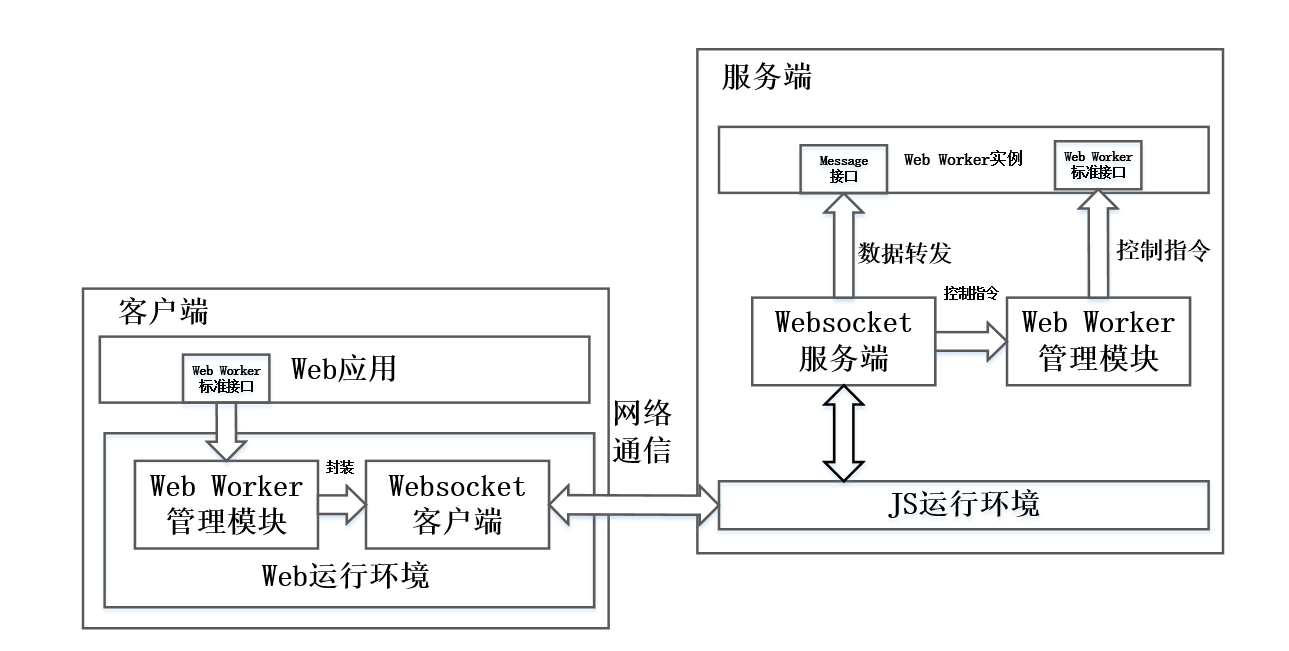
\includegraphics[width=1.0\textwidth]{Computation_Offloading_Web_Worker_Trans_Temp}
    \caption{Web Worker透明计算迁移}
    \label{fig:computation_offloading_web_worker_trans}
\end{figure}

\subsection{透明迁移的客户端}

% 这一部分介绍客户端结构、透明性、以及通信标志
客户端包含Web应用和重写的Web运行环境两个部分。Web运行环境在本研究中主要指运行在用户终端上的Web浏览器,它能够为HTML5及Javascript提供标准支持。因为设计的计算迁移系统为透明迁移,所以Web应用只需要调用标准的Web Worker接口就可以生成Web Worker并与其进行通信,而不需要对Web应用本身做任何特殊的改动,Web应用开发者也不需要了解底层是如何实现的。底层的Web运行环境被重新改写,主要包含Web Worker管理端和WebSocket通信客户端。当系统决定要进行计算迁移的时候,Web Worker管理端在收到上层Web应用通过标准接口传来的Web Worker生成的请求的时候,会将该请求进行翻译并重新封装,Web运行环境中的WebSocket通信客户端模块会通过WebSocket将封装后的请求发送到服务端进行处理。

在后续的通信中,客户端与运行在服务端的Web Worker要进行很多信息交互,这些通信也是以WebSocket的形式进行的,因此需要为WebSocket设置几种通信标志,来区分不同的通信类型。本研究中主要设置三种通信标志:
\begin{itemize}
    \item ESTABLISH:客户端请求服务端创建新的Web Worker,由服务端直接进行处理
    \item COMMUNICATE:客户端向服务端发送的通信信息,由服务端接收后转发给服务端对应的Web Worker
    \item TERMINATE:客户端请求服务端停止对应的Web Worker,由服务端直接进行处理
\end{itemize}

添加通信标志的操作是在客户端中的WebSocket通信客户端重新封装请求的过程中实现的。这些通信标志可以让服务端区分该信息是控制类型(ESTABLISH、TERMINATE)还是数据类型(COMMUNICATE),并根据通信类型的不同采取不同的处理方式。

\subsection{基于容器的服务端}

% 这一部分介绍服务端结构、容器集群以及整个流程,包括论文里的迁移的4个阶段
图\ref{fig:computation_offloading_web_worker_trans}中右侧为服务端程序的模块。服务端程序包括底层的Javascript运行环境、WebSocket通信服务端以及Web Worker管理端。Javascript运行环境用来提供Javascript标准接口,支撑整个服务端程序以及Web Worker的运行。WebSocket通信服务端用来接收客户端发来的消息,并且对其解封装,根据通信标志的不同,做相应的处理。Web Worker管理端,接收通信服务端传来的指令,调用Web Worker标准接口,实现对Web Worker生命周期的管理,包括Web Worker的创建、信息交互及销毁。

\begin{figure}[!htbp]
    \centering
    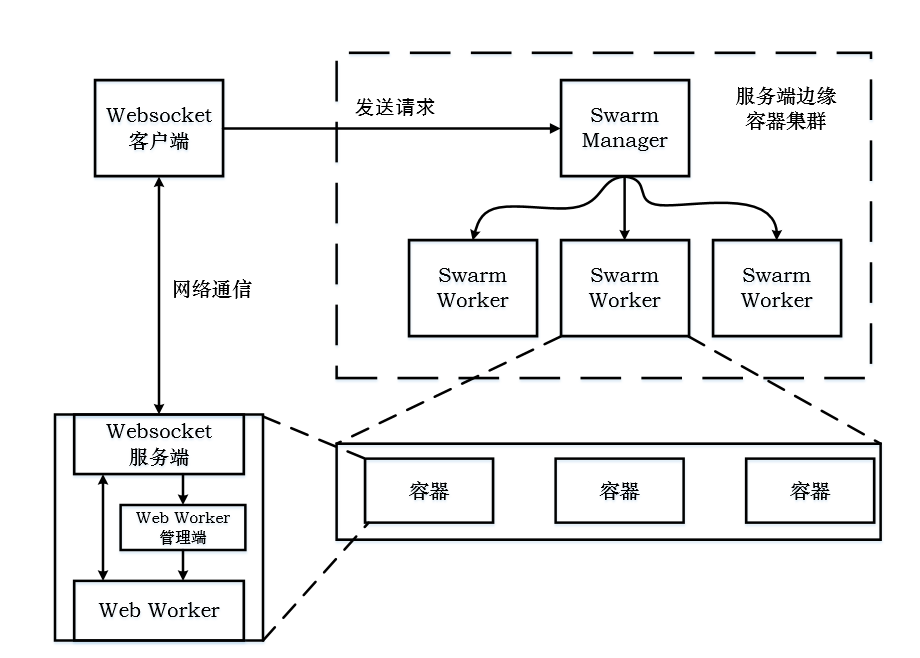
\includegraphics[width=1.0\textwidth]{Computation_Offloading_System_Server_Temp}
    \caption{透明计算迁移系统服务端结构图}
    \label{fig:computation_offloading_system_server}
\end{figure}

图\ref{fig:computation_offloading_system_server}为整个系统的整体架构图。服务端程序是以容器的形式部署在边缘Docker Swarm集群上的。这个过程需要使用Dockerfile生成安装有对应运行环境及服务端程序的Docker镜像,并将生成的镜像上传到本地镜像仓库中。
% dockerfile这里可以贴一下?
接下来需要由Docker Swarm集群从镜像仓库中拉取对应镜像,按照对资源以及服务规模的需求生成相应的迁移服务,并通过Docker Swarm的调度器在合适的终端节点上启动相应数量的副本实例,也就是运行着服务端程序的容器,打开对应端口,为用户终端提供计算迁移服务。每个容器在哪个节点上运行是由Docker Swarm调度器上执行的调度策略来决定的。

计算迁移的过程被分为4个阶段,运行时准备阶段,网络连接阶段,数据传输阶段,任务执行阶段。在运行时准备阶段中,服务端使用Dockerfile生成安装有对应运行环境及服务端程序的Docker镜像,或者直接从本地镜像仓库中下载对应镜像,创建对应服务,在节点上部署对应容器,并对外暴露服务端口。在网络连接阶段中,客户端接收到用户请求,Web应用根据用户请求向底层Web运行环境发送Web Worker的创建请求,客户端的Web Worker管理端会将带有创建Web Worker所需要的信息的JS文件的URL加上一个ESTABLISH标志,封装后交给客户端的WebSocket客户端。此时WebSocket客户端会向服务端暴露出的服务IP和端口请求建立连接,通过服务端Docker Swarm的调度以后,客户端与某个容器上运行的服务端的WebSocket服务端端建立网络连接。WebSocket服务端在接收到消息后会进行解封装,读取通信类型标志并根据消息内容中包含的URL下载对应JS文件。然后服务端上的Web Worker管理端会在对应容器中运行该JS文件,创建Web Worker。在数据传输阶段中,WebSocket客户端发送的信息带有COMMUNICATE通信标志,代表信息中包含的内容是Web应用发送给Web Worker的数据信息,WebSocket服务端解析到该标志后,会直接将信息转发给在容器中运行的Web Worker。在任务执行阶段中,运行在边缘容器中的Web Worker会利用容器中配置的资源,执行对应计算任务,并将计算结果通过网络返回给用户的客户端设备。当该客户端接收到某个Web Worker返回的全部数据,则会向该服务端发送带有TERMINATE标志的信息,服务端在接收到该消息后,会销毁对应容器中运行的Web Worker,释放相关资源。此时该容器并不会随之销毁,而是可以等待下一次计算迁移任务,直到整个Docker Swarm集群对该容器的生命周期进行调整。

% \subsection{流程}
% 这一章应该比较好写,就把之前的实验报告怼上去就行
\section{实验结果及分析}\label{sec:computation_offloading_experiment_results}

\subsection{实验配置}

本研究中使用树莓派设备来模拟用户终端设备及边缘终端设备,搭建基于容器的Web Worker透明边缘计算迁移系统,并测试其对于用户服务体验的提升效果。本实验中的客户端以及服务端集群使用的树莓派型号为raspberry pi3,配置为1G内存,4核处理器。服务端Docker Swarm集群由局域网内的4个树莓派组成,其中一个作为master,另外三个作为worker,每个树莓派节点上都可以作为计算迁移服务的执行节点。另外为了与基于容器的边缘集群的性能做对比,还使用了一台局域网内的Dell PowerEdge R730服务器作为服务端来进行实验。本实验中客户端的Web运行平台为chromium浏览器,服务端的JS执行环境为基于V8引擎的Node.JS。

本实验中的测试用例为利用一个利用Web Worker的图形渲染Web应用Ray Tracing (http://nerget.com/rayjs-mt/rayjs.html)。在这个实验中,Web应用需要渲染加载一张图片,具体过程是将图片切割成若干份(本实验中为20份),启动一定数量的Web Worker来进行渲染加载。这个测试用例中,图片的大小是一定的,也就是总的任务量一定,使用的Web Worker数量越多,每个Web Worker计算的任务量就越少,同时Web Worker数量与切割份数不一定相同,可能出现一个Web Worker需要处理多个任务的情况。在本实验中,Ray Tracing应用可以不做任何修改,直接运行在客户端树莓派的chromium上,这体现了所提出的的计算迁移技术的透明性。经过修改后的chromium浏览器将计算任务迁移到边缘树莓派集群或服务器上,创建Web Worker并进行计算,最后将结果返回给客户端,浏览器将图片显示给用户。本实验中对基于容器的Web Worker透明边缘计算迁移系统服务性能的评价指标为Web Worker的总体执行时间,即从第一个Web Worker开始创建,到最后一个Web Worker执行完成所消耗的时间。

\subsection{实验结果}

为了测试不迁移、迁移到服务器以及迁移到边缘树莓派集群上的服务性能,本研究完成了容器集群迁移性能测试实验。在本实验中图片大小为200*200,切分为20份200*10的小图片,交给不同数量的Web Worker来进行计算,实验结果如图\ref{fig:computation_offloading_result_picture_200}所示,其中横坐标表示每一次实验中的Web Worker数量,纵坐标表示该次实验中的Web Worker执行总时间。

\begin{figure}[!htbp]
    \centering
    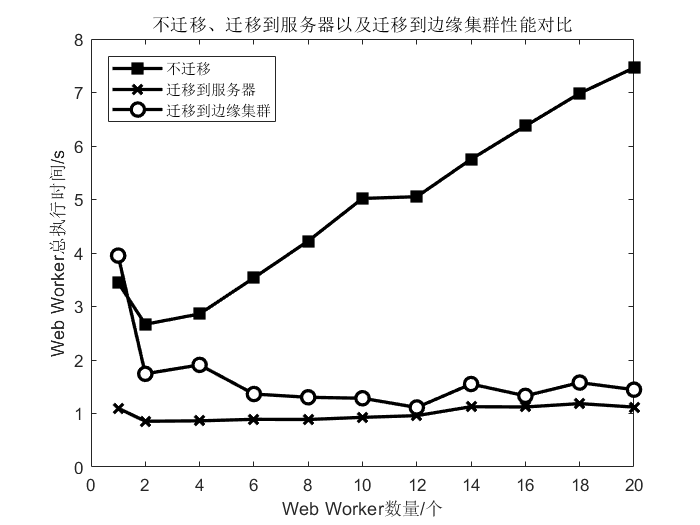
\includegraphics[width=0.8\textwidth]{offloading200}
    \caption{容器集群迁移性能测试实验}
    \label{fig:computation_offloading_result_picture_200}
\end{figure}

从图\ref{fig:computation_offloading_result_picture_200}中可以看出,当不使用计算迁移系统的时候,执行总时间最长,服务性能最差,而且随着Web Worker数量的增加,计算执行时间大大增加,用户服务体验显著变差。当迁移到边缘树莓派集群上的时候,相比不进行计算迁移的情况,终端服务质量提升明显,虽然总计算执行时间比迁移到服务器的情况稍差,但相差不是很显著,还是能够保持在用户可接受范围内。另外随着Web Worker数量的增加,迁移到边缘树莓派集群的执行总时间会慢慢增加,但增长趋势比较缓慢,相比不进行计算迁移的情况拥有较好的服务质量控制能力。当Web Worker数量为20的时候,不进行计算迁移时候的总执行时间为7.461秒,透明迁移到边缘树莓派集群时候的总执行时间为1.445秒,优化效果为80.6\%。
当迁移到服务器上的时候,计算执行时间最短,尤其是在Web Worker数量为1的时候,效果非常明显,但这更多的是基于服务器本身性能要远远好于单个树莓派的原因。在实际应用场景中,使用服务器来提供计算迁移服务的成本要远远高于使用边缘终端设备,而且在实际的应用场景中,服务器通常位于云端数据中心,距离用户终端设备较远,网络通信开销会增大,同时还会受限于网络状况,服务性能很可能达不到实验预期的效果。

为了测试透明迁移到边缘树莓派集群与非透明迁移到集群的服务性能差异,本研究完成了透明计算迁移性能测试实验。在本实验中,图片大小为400*400,切分为20份400*20的小图片,交给不同数量的Web Worker来进行计算,实验结果如图\ref{fig:computation_offloading_result_picture_400}所示,其中横坐标表示每一次实验中的Web Worker数量,纵坐标表示该次实验中的Web Worker执行总时间。

\begin{figure}[htbp]
    \centering
    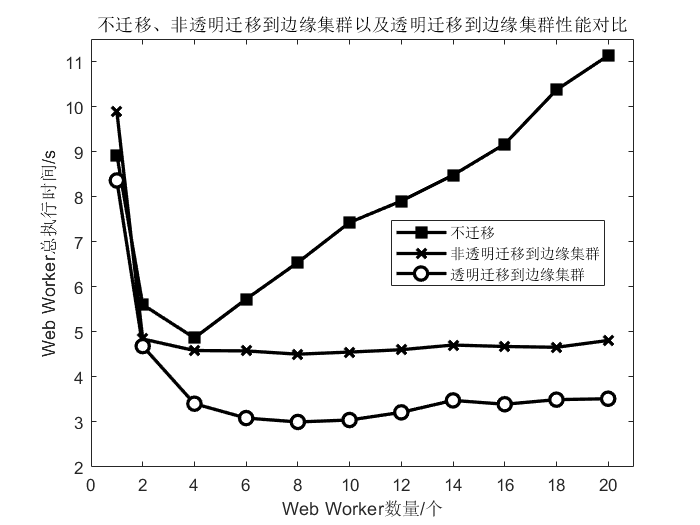
\includegraphics[width=0.8\textwidth]{offloading400}
    \caption{透明计算迁移性能测试实验}
    \label{fig:computation_offloading_result_picture_400}
\end{figure}

从图\ref{fig:computation_offloading_result_picture_400}中可以看出,相比容器集群迁移性能测试实验,图片大小变大,总任务量变多,总的计算时间也相应增加。相比其他两种计算迁移方式,不使用计算迁移系统的情况的计算执行总时间最长,服务质量最差,而且随着Web Worker数量的增加,计算时间大大增加,用户的服务体验显著变差。当Web Worker数量为20的时候,不进行计算迁移时候的总执行时间为11.131秒,透明迁移到边缘树莓派集群时候的总执行时间为3.515秒,性能提升68.4\%。
另外值得注意的一点是,在不使用计算迁移系统的情况下,当使用4个Web Worker来执行任务的时候,总计算执行时间最短,这可能与树莓派设备是4核处理器有关,当Web Worker数量小于4个的时候,会出现树莓派的计算能力没有被充分利用的情况,当Web Worker数量大于4个的时候,会出现因各个线程之间抢占CPU而导致切换时间大大增加影响总执行时间的情况。当使用计算迁移进行计算的时候,总的执行时间都会大大缩短,尤其是当Web Worker数量多于4个的时候,服务性能优化效果十分明显,这也是基于边缘树莓派集群中拥有多设备多核处理器的原因。当Web Worker数量增加的时候,总执行时间也不会随之增加很多,稳定在一个比较短的时间内。对比透明计算迁移方式和非透明计算迁移方式的实验结果,可以看出,透明计算迁移方式的总执行时间也要比非透明计算迁移方式的总执行时间要短一些,整体服务效果更好。当Web Worker数量为8的时候,使用非透明计算迁移方式的计算执行总时间为4.551秒,使用透明计算迁移方式的计算执行总时间为3.000秒,性能提升33.1\%。

\section{本章小结}\label{sec:computation_offloading_summary}

传统的终端设备的服务模式通常是终端设备在本地进行计算任务的运行,依靠终端设备自身的计算能力来保证服务质量。而随着边缘智能终端设备所要承担的计算任务越来越重,单一终端设备本地计算难以满足终端服务和任务对终端计算能力的要求,计算迁移技术逐渐成为了一个可行的解决方案。在基于容器化多终端协同服务技术中,计算迁移技术成为将用户周围终端设备上的空余资源利用起来,为用户提供协同服务的具体实现方式。

本章基于多终端协同服务技术的应用场景,提出了一种基于容器的Web Worker透明边缘计算迁移技术。本章通过重新设计开发客户端Web运行环境,改写其中的Web Worker相关接口,在对上层Web应用保持透明的情况下,利用WebSocket将生成Web Worker的请求发送到服务端进行计算,实现了Web Worker的透明计算迁移。另外,利用Docker Swarm容器集群,将透明计算迁移的服务端部署到用户周围的边缘终端上面,方便对边缘终端设备的空余资源进行管理和利用。本章通过两个实验证明所提出的基于容器的Web Worker透明边缘计算迁移技术可以很好地利用用户周围的边缘终端设备的空余资源,相比不使用计算迁移、直接在本地进行计算的方式,可以大大减少Web Worker的总执行时间,当Web Worker数量增加的时候,也能够将Web Worker总执行时间的增长情况控制在一个相对很小的水平。实验结果表明,所提出的基于容器的Web Worker透明边缘计算迁移技术,对于减少Web应用中Web Worker的总执行时间,提高用户体验有着很显著的效果。

本章所涉及的研究成果包括:

论文1篇:“基于容器的Web Worker透明边缘计算迁移系统”(核心期刊,在投)。